\chapter{実験}
ここでは本研究において行った実験について述べる.

\section{実験1ドライブレコーダー映像を利用した実験}
\subsection{実験内容}
本研究における最初の本実験として、予備実験をもとに実装したシステムを実際にドライブレコーダー映像を使って検証した。
また、strct2depth画面における車のbbox内のG値が100を超えた際に渋滞と判断し、画面左上に「Traffic Jam」という文字列が表示されるようにした。
加えて、映像中に渋滞が判断された回数をフレームごとにJam Counterとして回数を映像中段左に表示されるようにした。

\subsection{使用したデータセット}
本実験にて使用したデータセットは動画投稿サイトYouTubeにて公開されていた高速道路を走行中の映像に加え、私の家族が使用している自家用車に取り付けられたドライブレコーダー映像を用いる。

% 実験1で発生した問題を述べる
\section{実験結果と課題}
ここでは実験1における実験結果について問題と考察を述べる.
まず、実験1における実験結果を以下に示す。
実験結果1〜3の通り、予備実験にて改良したシステムをそのまま用いると、様々な状況で渋滞を誤検出するという問題が発生してしまう。
% --------------------------------------------------
\newpage
\begin{figure}[htbp]
  \begin{tabular}{c}
    \begin{minipage}{0.33\hsize}
      \begin{center}
   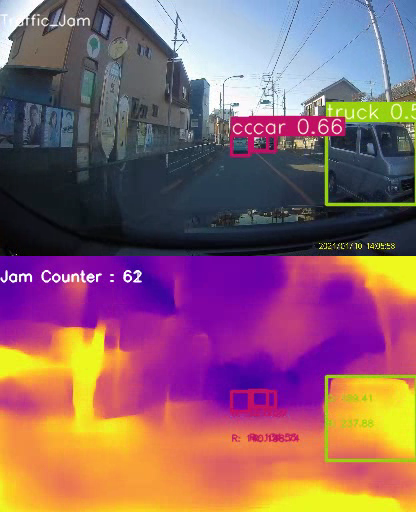
\includegraphics[width=4.5cm]{figs/ex01_01.png}
    \end{center}
  \caption{結果1 対向車線の車を検出し、渋滞だと判断してしまう。}
  \label{fig:ex01_01}
\end{minipage}

  \begin{minipage}{0.33\hsize}
  \begin{center}
    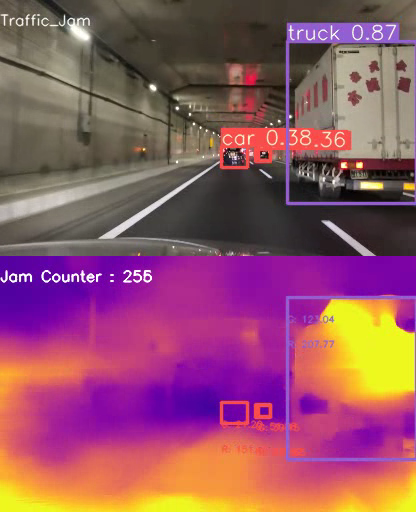
\includegraphics[width=4.5cm]{figs/ex01_02.png}
  \end{center}
  \caption{結果2 隣の車線の自動車を検出し、渋滞だと判断してしまう。}
  \label{fig:ex01_02}
\end{minipage}

  \begin{minipage}{0.33\hsize}
  \begin{center}
    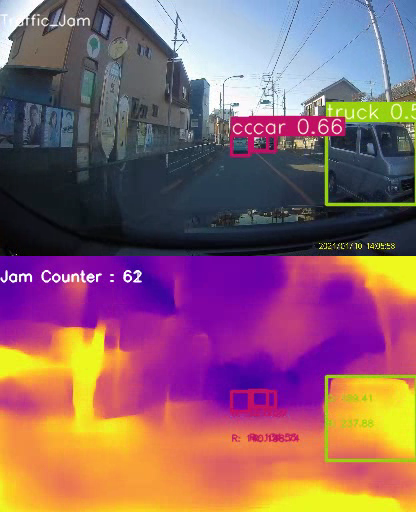
\includegraphics[width=4.5cm]{figs/ex01_01.png}
  \end{center}
  \caption{結果3 道路の脇に停車しているトラックを検出し、渋滞だと判断してしまう.}
  \label{fig:ex01_03}
\end{minipage}
\end{tabular}
\end{figure}

% ---------------------------------------------------

\subsection{隣の車線の車を検出してしまう問題}

\subsection{解決アプローチ}

\section{実験2}

\section{実験結果}


